%\documentclass[12pt]{article}    % <--- 12pt font
%\usepackage[margin=1in]{geometry}% <--- 1 in margin
                  % <--- double space
\documentclass[12pt]{amsart}
\usepackage[utf8]{inputenc}
\usepackage[a4paper,margin=1in,footskip=0.25in]{geometry}
\usepackage{setspace}
\doublespace    
% See geometry.pdf to learn the layout options. There are lots.
\geometry{letterpaper}                   % ... or a4paper or a5paper or ... 
%\geometry{landscape}                % Activate for for rotated page geometry
%\usepackage[parfill]{parskip}    % Activate to begin paragraphs with an empty line rather than an indent
\usepackage{float}
\usepackage{graphicx}
\usepackage{amssymb}
\usepackage{epstopdf}
\usepackage{amsmath}
\newtheorem{thm}{Theorem}
%\usepackage{algorithm}
\usepackage{subfig}
\usepackage[authoryear]{natbib}
%\usepackage{subcaption}
\usepackage[ruled,vlined]{algorithm2e}
%\linespread{1.5}
\usepackage{comment}
\usepackage{booktabs}
\usepackage{listings}
\usepackage{color}

\definecolor{dkgreen}{rgb}{0,0.6,0}
\definecolor{gray}{rgb}{0.5,0.5,0.5}
\definecolor{mauve}{rgb}{0.58,0,0.82}

\lstset{frame=tb,
  language=python,
  aboveskip=3mm,
  belowskip=3mm,
  showstringspaces=false,
  columns=flexible,
  basicstyle={\small\ttfamily},
  numbers=none,
  numberstyle=\tiny\color{gray},
  keywordstyle=\color{blue},
  commentstyle=\color{dkgreen},
  stringstyle=\color{mauve},
  breaklines=true,
  breakatwhitespace=true,
  tabsize=3
}


\usepackage[colorlinks=true,linkcolor=blue, allcolors=blue]{hyperref}%


\begin{document}
\author{Chris Chen}
\author{Peter Liu}
\author{Yuchen Sun}
\author{Yueqi Xu}
\title{Method Review of the BNT162b2 Vaccine Phase III Trial}

\begin{abstract}
\begin{comment}
In December of 2020, BioNTech and Pfizer published their phase III clinical trial results on the BNT162b2 mRNA Covid-19 vaccine efficacy. Succeeding their publication is an ongoing debate on the Bayesian methods used to arrive at their results. Using the same dataset, this paper implements both frequentists and bayesian methods to arrive at comparable results and comment on the validity of each method.   

\end{comment}
In this project, we analyze the vaccine efficacy of BNT162b2 via both Bayesian and Frequestist approaches. We propose multiple prior selection methodologies, and cross-compare them with popular Frequestist methods such as likelihood ratio test and Clopper-Pearson interval. We elaborate the strength and weakness of the proposed methods and critically analyze the prior choice in \cite{paper}. We further provide our own prior selection philosophy, which we consider more justifiable than that of \cite{paper}.
\smallskip

\noindent \textbf{Keywords.} COVID-19, Vaccine Efficacy, Bayesian, Frequentist, Prior Selection
\end{abstract}

\maketitle
\section{Introduction}
\label{sec: intro}
Coronavirus disease 2019 (Covid 2019), a contagious disease caused by severe acute respiratory syndrome coronavirus 2 (SARS-CoV-2), continues to rage in a worldwide pandemic. A return to normality has increasingly come to rely on the research and development of safe and effective vaccines.
\begin{comment}, especially in countries or regions that have been unable or unwilling to institute strong public health measures. 
\end{comment}

In 2020, BioNTech and Pfizer conducted an multinational, placebo-controlled, observer-blinded, pivotal efficacy trail, which randomly assigned persons 16 years of age or older in a 1:1 ratio to receive two doses, 21 days apart, of either placebo or the BNT162b2\footnote{A lipid nanoparticle–formulated, nucleoside-modified RNA 
vaccine that encodes a prefusion stabilized, membrane-anchored SARS-CoV-2 fulllength spike protein.} vaccine candidate. In the efficacy analysis at the first primary endpoint, among 36523 participants who had no evidence of existing or prior SARS-CoV-2 infection, 8 cases of laboratory-confirmed Covid-19 with onset at least 7 days after the second dose were observed among vaccine recipients and 162 among placebo recipients.

A Bayesian beta-binomial model with a minimally informative prior is used for primary efficacy endpoint. \cite{paper} proposed a beta prior with shape parameters $(0.700102, 1)$ for $\theta = (1 - \psi) /(2 - \psi)$, where $\psi$ is the vaccine efficacy (VE). The prior is centered at $\theta = 0.4118$, corresponding to VE = 30\%, which was claimed to be pessimistic. Their result shows BNT162b2 was 95\% effective in preventing Covid-19, with a 95\% Credible interval of $[90.3\%, 97.6\%]$.

In this project, we will attempt to answer the following question: ``\textit{What will be a proper statistical methodology to analysis vaccine efficacy?}" We will draw from the tools and knowledge we learned throughout the STAT 34x sequence to investigate issues such as prior choice and to compare with Bayesian and Frequentist methods.

\begin{comment}
This project critically examines the choice of statistical methods in \cite{paper}. 
\end{comment}


\begin{comment}
We will make three contributions in this work. First, we will examine the quality of the proposed prior in \cite{paper} by comparison with different choices of minimally informative or uninformative priors. Then, dual to Bayesian approaches, we will further analyze the vaccine efficacy using Frequestist methods, i.e. likelihood ratio test (LRT), Clopper–Pearson method, etc. Lastly, in later discussion, we will cross compare the results from the two methodologies, elaborate their benefits and shortcomings, and critically analyze the effectiveness of the Bayesian design in \cite{paper}.


The paper is structured as follows. In Section \ref{sec: meth}, we will elaborate the methodology
\end{comment}


\section{Methodology}
\label{sec: meth}
We will now outline the general problem we consider. Denote $X$ as the number of cases of Covid-19 infection among vaccine recipients and $Y$ among placebo recipients. Heuristically, suppose all trials are independent, and the probability of being infected with Covid-19 are consistent across all subjects within each group. A reasonable binomial model for $X, Y$ is
\begin{align}
    X \sim Binom(n_1, \pi_1), \quad Y \sim Binom(n_2, \pi_2), \quad X \perp Y, 
\end{align}
where $\pi_1, \pi_2$ are the infection probability across vaccine and placebo group with sizes $n_1 = 17,411$ and $n_2 = 17,511$ respectively. 
The vaccine efficacy (VE), which is defined in \cite{paper} as
\begin{align}
    \psi \equiv 1 - \frac{\pi_1}{\pi_2},
\end{align}
is our parameter of interest. Note that, the maximum of $\psi$ is attained at 1 (when $x = 0$), whereas the minimum is attained at minus infinity (when $y = 0$, $x > 0$), so that $\psi \in (-\infty, 1]$. Given this nature, directly doing inference on $\psi$ can be intractable.

\cite{paper} shied away from analyzing $\psi$ directly and considered a transformation of $\psi$ as an alternative. Now, Denote $W = X|X+Y=n$, where $n$ is the observed infected cases from all subjects. Given large sample sizes and low event rate, the binomial distribution of $X, Y$ can be approximated by a Poisson distribution with $\lambda_1 = n_1\pi_1$ and $\lambda_2 = n_2\pi_2$. Under such an approximation, the distribution of $W$ will follow as
\begin{align}
    W \sim Binom \left(n, \theta = \frac{n_1\pi_1}{n_1\pi_1+n_2\pi_2}\right).
\label{eq: W}
\end{align}
A simple derivation of the distribution of $W$ will be given in Appendix \ref{sec: 4intervals}. In the vaccine trial, due to 1:1 randomization, approximately we have $n_1 \approx n_2$. Thus, a heuristic expression of $\theta$ is
\begin{equation}
  \theta =\frac{n_1\pi_1}{n_1\pi_1+n_2\pi_2} \approx \frac{\pi_1}{\pi_1 + \pi_2} = \frac{1 - \psi}{2 - \psi}. 
  \label{eq:theta-psi}
\end{equation}
%and correspondingly
%\begin{equation}
%  \psi = \frac{1-2\theta}{1-\theta}. \label{eq:psi-theta}
%\end{equation}
Indeed, given a fixed number of observed cases, $\theta$ can be considered as the probability of a randomly chosen case will be in the vaccine group. After transformation, $\theta$ takes the form of a binomial proportion, which immediately enables prevalent Frequestist and Bayesian methods, which we will elaborate as follows.

\subsection{Bayesian Workflow}

The binomial model enjoys a conjugate prior with the form of a Beta distribution with $\alpha, \beta$ being the first and second shape parameters. The corresponding posterior follows a Beta-binomial distribution
\begin{align}
    W|X, n, \theta, \alpha, \beta \sim Beta (\alpha + X, \beta + n - X).
\end{align}
Selecting a proper prior is the cornerstone of any Bayesian workflow. We will now introduce four philosophies for prior selection. 
\subsubsection{Uninformative Priors}
We will first propose two uninformative priors that does not incorporate subjective belief from practitioners, namely the Flat prior and the Jeffreys prior. The Flat prior considers the probability of each parameter being selected is uniformly distributed across the parameter space, which is 
$   \theta \sim Beta(1, 1) \equiv Unif(0, 1).
    \label{pri: flat}$
    
The Jeffreys prior is another prevalent choice of uninformative prior in Bayesian analysis. In the case of Beta-binomial model, the Jeffreys prior takes the form of
$    \theta \sim Beta(1/2, 1/2).
    \label{pri: Jef}$
    
Note that, for binomial model, the data has the least effect on the posterior when $\theta_{\text{true}} = 1/2$, and has greatest effect near the extremes, that is, when $\theta_{\text{true}} = 0 \text{ or } 1$, which is very likely in the vaccine efficacy trial. The Jeffreys prior compensates for this by placing more mass on the extremes and less mass in the middle. See Figure \ref{fig: uninformative} for a visualization of the Jeffreys prior for binomial model.

\subsubsection{Mean \& Variance Based Beta Priors}
\label{sec: 212}
\cite{paper} proposed a minimally informative prior with a prior belief on an average vaccine efficacy of 30\%. Minimally informativeness can be consider in regard to the variance of prior distribution. More specifically, the weaker the prior belief, the larger the variance, the less informative the prior is. Prior belief on vaccine efficacy is incorporated by \cite{paper} as follows: by transformation in (\ref{eq:theta-psi}), a VE of $30\%$ corresponds to a $\theta = 0.4118$. Thus correspondingly, the mean of $\theta$ is set as $\mu_\theta = 0.4118$. Then, by straight-forwardly specifying $\beta = 1$\footnote{For $\mathbb{E}[\psi] < \infty$, it is required that $\beta > 1$. However, prior choices with $\beta \leq 1$ can also be considered as valid.}, a set of desired parameters of the beta prior is obtained by solving $\mu_\theta = \alpha / (\alpha + \beta)$, which yields
\begin{align}
    \theta \sim Beta(0.700102, 1).
    \label{pri: paper}
\end{align}

Such a prior choice, with a variance of $0.0901$, allows considerable uncertainty. The $95\%$ interval for $\theta$ is $[0.005, 0.964]$, with the corresponding $95\%$ interval for VE to be $[-2620\%, 99.5\%]$. In this case, naively choosing $\beta = 1$ results in a desired minimally informative prior with large variance. However, this may not be true in general and can be problematic in practice. 

We will now propose a generalized prior selecting procedure based on \cite{paper} with a user-defined VE average $\mu_\psi$ and variance $\sigma^2$. We will first transform $\mu_\psi$ into $\mu_\theta$ accordingly by (\ref{eq:theta-psi}). Now, a desired beta prior on $\theta$ will follow as
\begin{align}
    \theta\sim Beta\left(\frac{\mu_\theta^2 (1 - \mu_\theta) - \mu_\theta \sigma^2}{\sigma^2}, \frac{(1 - \mu_\theta)(\mu_\theta^2 (1 - \mu_\theta) - \mu_\theta \sigma^2)}{\mu_\theta \sigma^2}\right).
    \label{pri: var}
\end{align}
Such a prior will enable practitioners to control the mean and informativeness of the beta prior. A visualization of the relationship between informativeness and variance can be found at Appendix Figure \ref{fig:my_label}.

\subsubsection{Single Quantile \& Variance Based Beta Priors}
\label{sec: 213}
An alternative way to incorporate prior belief is via specifying the quantile of prior distribution. Echo to mean based methods in Section \ref{sec: 212}, we will propose a prior selecting procedure with a user-defined VE quantile $q_\psi$ and variance $\sigma^2$. 

Similarly, we will first transform $q_\psi$ into $q_\theta$. Note that, unlike the previous case, given $q_\theta$ and $\sigma^2$, there are no closed form solutions for $(\alpha, \beta)$. Thus, a grid approximation is used to find a desired set of the shape parameters. The algorithm will scan through a fine grid of a subset of $\mathbb{R}^2$, and will stop if the differences in quantile and variance are less than a desired threshold. An \texttt{R} code implementation can be found in Appendix \ref{code: grid}.

\subsubsection{Double Quantile Based Beta Priors} 
\label{sec: 214}
\begin{comment}
In many applications, informative priors can be more beneficial. We will propose two methodologies to construct priors that incorporate prior belief. 
\end{comment}
Apparently, the prior belief can be interpreted via more than one quantile. Suppose for now that the practitioners express their prior beliefs over two quantile of vaccine efficacy, namely $q_{\psi, 1}$ and $q_{\psi, 2}$. Our first step will continue to transform $(q_{\psi, 1}, q_{\psi, 2})$ to $(q_{\theta, 1}, q_{\theta, 2})$. A desired choice of beta prior is then computed using
the $\texttt{LearnBayes::beta.select}$ function in $\texttt{R}$. More specifically, in this vaccine trial, we will provide a prior choice based on our own belief, which will be speculated in the following manner: 
\begin{enumerate}
  \item The median of vaccine efficacy is $0$. Thus $\theta$ has a median of $0.5$;
  \item The $95th$ percentile of vaccine efficacy is $0.3$. Thus the $5th$ percentile of $\theta$ is $0.4118$.
\end{enumerate}
Such a prior can be considered more pessimistic than the prior proposed in \cite{paper}. Moreover, it reflects a strong prior belief, with a variance of $0.0029$.

In later result and discussions, we will elaborate the strength and weakness of these priors, and cross compare their estimation performances.
\begin{comment}
At the end of the day, we wish to study how the strength of prior belief, in term of variance, will impact the behavior of credible interval.
\end{comment}
\subsection{Frequestist Workflow}
We will further introduce two Frequestist approaches reciprocal to the Bayesian analysis.
\subsubsection{Confidence Interval for Binomial Proportion}

\cite{paper} considered the Clopper-Pearson method to construct confidence interval (CI) for the binomial proportion $\theta$. The CI is directly converted upon vaccine efficacy via transformation (\ref{eq:theta-psi}). The Clopper-Pearson CI guarantees the coverage rate is at least the nominal confidence interval by inverting the acceptance regions based on the exact p-value corresponding to the binomial distribution. This is a prevalent choice to analyze binomial proportion and is the default of $\texttt{mosaic::binom.test}$ in \texttt{R}.

Clopper-Pearson method in \cite{paper} yields an average of $95.0\%$ for VE and a $95\%$ CI of $[90.0\%, 97.9\%]$.
Given the sample size is relatively large, we will further propose three alternative CI methods to compare with the proposed Clopper-Pearson: the Wald method, the Wilson's Score method, and the Plus-4 method. These methods are all built-in functions in \texttt{R} and can be applied efficiently. Closed formed formulas and implementation details can be found in Appendix \ref{sec: 4intervals}. 
\begin{comment}
In general, there are four commonly used methods that calculate confidence intervals based on binomial proportion. Based on the fact that binomial converges to normal asymptotically when $n$ is large, we can use the Wald method. Using the connection between hypothesis tests and confidence intervals, we can derive the Wilson Score confidence interval. A good compromise between the Wald method and the Score method is the Plus-4 method, which is deriving by adding two successes and two failures to the sample data, and compute the Wald's interval. And the Clopper-Pearson confidence interval is computed by inverting the acceptance regions based on the exact p-value corresponding to the binomial distribution.
\end{comment}
 

\subsubsection{Likelihood Ratio Test} 

Likelihood Ratio Test (LRT) is a popular likelihood-based method that is widely used to perform hypothesis testing and to construct confidence interval. In our case, the hypothesis\footnote{Intuitively, the hypothesis should be $H_0: \psi \leq 0.3, H_1: \psi > 0.3$. However, this will not satisfy the dimension constraints of the common LRT. See \cite{CB} Example 8.2.6 for a LRT framework that may be applied on this hypothesis. In this project, we will take the hypothesis in (\ref{hypo}) for LRT heuristically.} concerning vaccine efficacy $\psi$ is
\begin{align}
    H_0: \psi = 0.3, \quad H_1: \psi \neq 0.3 \;. 
    \label{hypo}
\end{align}
By transformation via Equation (\ref{eq:theta-psi}), the pair of hypothesis can be re-written as
\begin{align}
    H_0: \theta = 0.4118, \quad H_1:  \theta \neq 0.4118 \;.
\end{align}
Given the binomial model, the MLE of $\theta$ has the closed form solution
    $\widehat{\theta}_{MLE} = W / n,$
thus the likelihood ratio is 
\begin{align}
    \lambda = \frac{L(\theta_0)}{L(\widehat{\theta}_{MLE})} = \frac{(\theta_0)^w(1-\theta_0)^{n-w}}{(\widehat{\theta}_{MLE})^w(1-\widehat{\theta}_{MLE})^{n-w}}.
\end{align}
The binomial model for efficacy data enjoys a smooth likelihood function, a relatively large sample size, and a support that is invariant of choices of $\theta$. Thus, by Theorem 2.1 of likelihood ratio lecture note, under the null hypothesis we have 
\begin{align}
    -2 \log (\Lambda)\stackrel{D}{\rightarrow} \textit{Chisq}(df=1).
\end{align}
The validity of such an approximation is provided in Appendix Figure \ref{fig: EmpPVal}. A $95\%$ confidence interval for $\theta$ can be calculated via 
\begin{align}
    - \log(\lambda) < qchisq(p = 0.95, df = 1).
\end{align}
% \clearpage

\section{Results \& data analysis}
\begin{figure}[H]
    \centering
    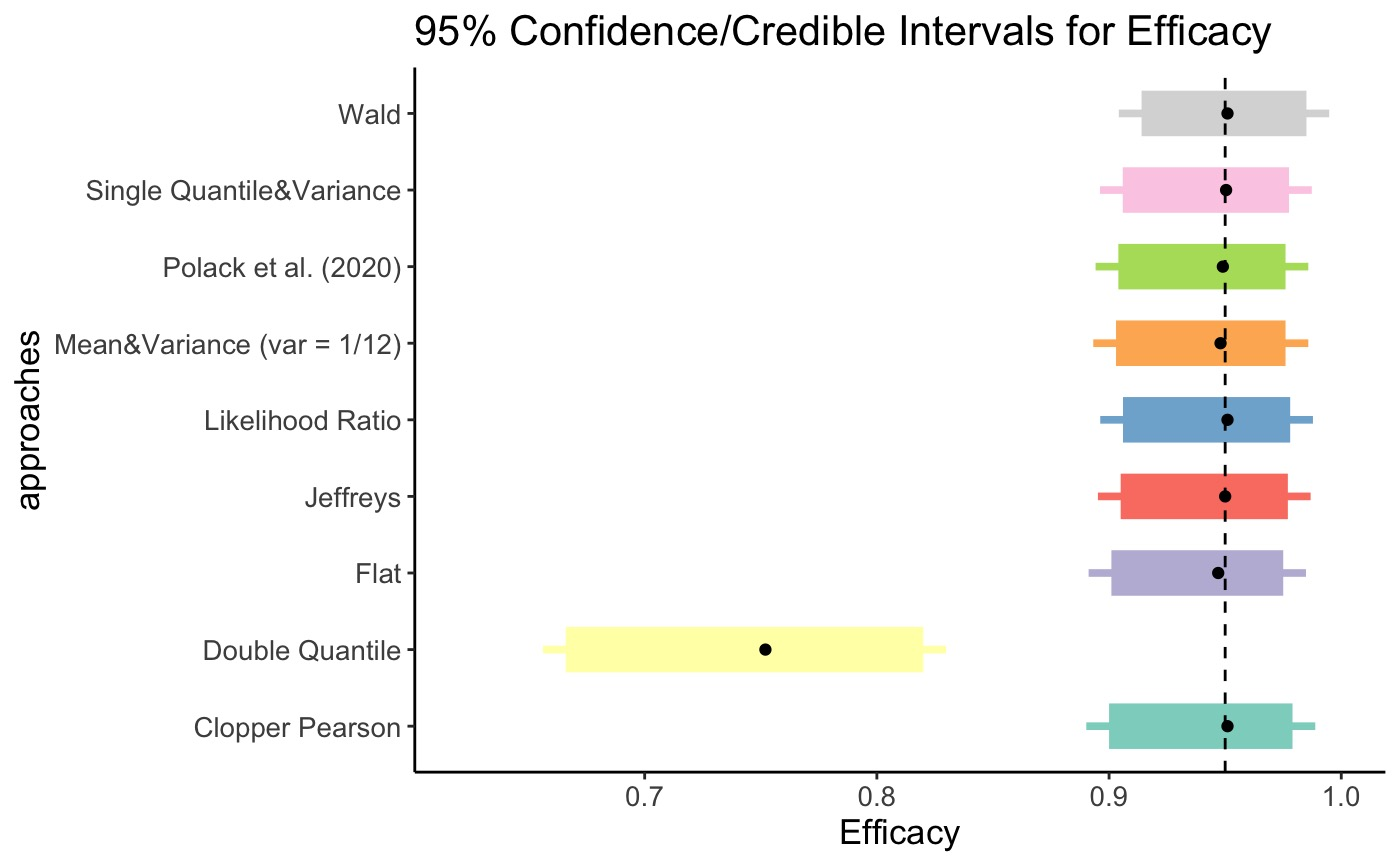
\includegraphics[width = 0.8\textwidth]{intervals.jpeg}
    \caption{\footnotesize{95\% Bayesian credible intervals and Frequentist CIs of vaccine efficacy.}}
    \label{fig: intervals}
\end{figure}
\subsection{Results for Bayesian Approaches}

\subsubsection{Uninformative Priors}
For the uninformative priors, we will not incorporate any prior information or beliefs on vaccine efficacy. With data dominating the posterior, the medians for $\psi$ should be close to Frequestist estimates. The median of Flat prior and Jeffreys prior are $94.7\%$ and $95.0\%$ respectively, which are quite close to the expected $95.1\%$ (with $\theta = 8/170$). Similarly,
the $95\%$ credible intervals of $\psi$ are very close, with a credible interval of $[90.1\%, 97.5\%]$ from flat prior and $[90.5\%, 97.7\%]$ from Jeffreys prior.

\subsubsection{Mean \& Variance Based Beta Priors}
We will consider two sets of parameters for this methodology.
First, we considered the proposed prior in \cite{paper} with $\alpha = 0.700102, \beta = 1$ (See Appendix Figure \ref{fig: weak}). The $95\%$ credible interval for $\psi$ is $[90.4\%, 97.6\%]$ and the posterior median is $94.9\%$.

Second, we considered an alternative prior proposed in \cite{blog}, satisfying $\theta$ = 0.4118 and a variance $\sigma^2 = 1 / 12$, which is the same as the variance of a Flat prior. Via calculation in Equation (\ref{pri: var}), we have $\alpha= 0.7852, \beta = 1.1215$. The corresponding 95\% credible interval is $[90.3\%, 97.6\%]$, which coincides with the 95\% credible interval of $\psi$ in \cite{paper}, with a posterior median of $94.8\%$. This is expected, since both priors are weakly informative with the same prior mean.

\subsubsection{Single quantile \& Variance Based Beta Priors}

We will consider a prior with a single quantile based prior belief as the median of VE is $50\%$. We will not specify a variance for this prior, and straightforwardly take $\beta = 1$, echoing the parameter choice in \cite{paper}. This corresponds to a beta prior with parameters $\alpha = 0.6293, \beta = 1$.  (See Appendix Figure \ref{fig: quantile}). The $95\%$ credible interval for $\psi$ is $[90.4\%, 97.7\%]$ and the posterior median is $94.9\%$.

\subsubsection{Double Quantile Based Beta Priors}
We will consider a strongly informative, pessimistic prior, which is elaborated in Section \ref{sec: 214}. This corresponds to the minimum VE requirement established by FDA and what we want to show how the VE is ``at least better than". We can observe the prior distribution, posterior distribution, and likelihood function have three unique peaks with the prior on the rightmost position and likelihood at the leftmost position (See Appendix Figure \ref{fig: strong}).

The $95\%$ credible interval of $\psi$ is $[66.6\%, 82.0\%]$, which is significantly distinct from other intervals and does not include $95.1\%$. Intuitively this makes sense, since our prior beliefs are very inconsistent with the observed data, which indicates our prior beliefs were being too pessimistic. However, note that the credible interval is still a lot greater than $30\%$, which implies VE is greater than 30\% with a probability at least of $95\%$.

\singlespacing
\begin{table}[H]
  \begin{center}
  \setlength{\tabcolsep}{10pt} % Default value: 6pt
\renewcommand{\arraystretch}{1.1}
    \begin{tabular}{ l l c c }
     Approach & Prior & Credible Interval & Median \\ \hline
     Jeffreys & $Beta(0.5, \, 0.5)$& $[90.5\%, 97.7\%]$ & $95.0\%$ \\ 
     Flat & $Beta(1, 1)$ & $[90.1\%, 97.5\%]$ & $94.7\%$ \\ 
     Double-Quantile & $Beta(43.06, \, 43.06)$ &  $[66.6\%, 82.0\%]$ & $75.2\%$ \\
     \cite{paper} & $Beta(0.700102, \, 1)$ & $[90.4\%, 97.6\%]$ & $94.9\%$ \\
     Mean \& Variance ($\sigma^2 = 1/12$) & $Beta(0.7852, \, 1.1215)$ & $[90.3\%, 97.6\%]$ & $94.8\%$ \\
     Single Quantile \& Variance & $Beta(0.6293, \, 1)$ & $[90.4\%, 97.7\%]$ & $95.0\%$ \\ \hline
    \end{tabular}
    \vspace{5pt}
    \caption{95\% credible intervals and medians of $\psi$ of different prior choices.} \label{table:1}
  \end{center}
\end{table}
\doublespacing
\subsection{Frequentist Approaches}
\subsubsection{Confidence Interval for Binomial Proportion}
We observed the Wald interval behaves worse than the Clopper-Pearson's because of the relatively small sample size $(n = 170)$, which results in less asymptomaticity. The 95\% confidence intervals of $\psi$ with different interval methods are provided in the table below.
\subsubsection{Likelihood Ratio Test}
The 95\% confidence interval of the likelihood ratio test is [90.6\%, 97.8\%], with a mean of 95.1\%. The validity of using a Chi-square approximation is verified using an empirical simulation with the p-value equals to 0.0002 (See Appendix \ref{fig: EmpPVal}).

\singlespacing
\begin{table}[H]
  \label{Tab: 2}
  \setlength{\tabcolsep}{10pt} % Default value: 6pt
\renewcommand{\arraystretch}{1.1}
  \begin{center}
    \begin{tabular}{ c c c }
     Approach & Confidence Interval & Mean \\ \hline
     Likelihood Ratio & $[90.6\%, 97.8\%]$ & $95.1\%$ \\  
     Wald & $[91.4\%, 98.5\%]$ & $95.1\%$ \\ 
     Score &  $[90.1\%, 97.5\%]$ & $95.1\%$ \\
     Plus-4 & $[89.9\%, 97.7\%]$ & $95.1\%$\\
     Clopper Pearson & $[90.0\%, 97.9\%]$ & $95.1\%$ \\ \hline
    \end{tabular}
    \vspace{2pt}
    \caption{95\% confidence intervals and means of $\psi$} \label{table:2}
  \end{center}
\end{table}
\doublespacing
\section{Discussion \& Conclusion}

We favor a Bayesian design over its Frequestist opponent attributed to the different statistical interpretations carried by the credible interval and confidence interval. A $95\%$ Bayesian credible interval $[c_{\min}, c_{\max}]$ of $\psi$ indicates that, given the observed data, the probability that the true $\psi$ is bounded by $[c_{\min}, c_{\max}]$ is $0.95$. In contrast, the boundaries of a $95\%$ Frequestist confidence interval does not carry any statistical meanings. The Frequestist CI can be interpreted in the following manner: ``\textit{were the vaccine trial repeated numerous times, the fraction of the calculated confidence intervals that encompass the true VE would tend towards 95\%} \citep{cox}.'' Thus, the Bayesian credible interval is preferred as it directly evaluates the probability of the true vaccine efficacy without assuming the vaccine trial were conducted repeatedly. 
\begin{comment}
Vaccine clinical trials is difficult to repeat multiple times because of ethical reasons.

Normally, clinical trials are stopped once a number of cases are observed. For safety reasons, the number of cases must be constraint to a minimal number to ensure most of the subjects remain healthy after the study. Therefore, although 43,548 total participants were invovled with the study, only 170 cases were observed and used as the sample size for further data analysis. When the sample size is small, Bayesian methods may be more effective in estimating the parameter. Bayesian method incorporates a prior belief and do not rely on asymptotics 

\textcolor{red}{https://www.tandfonline.com/doi/abs/10.1080/10705511.2016.1186549?journalCode=hsem20}(citation for bayesian do not rely on aymptotics).
\end{comment}

%More considerations need to be taken into account if we want to choose a method to construct the Bayesian credible intervals for $\psi$, in particular, the transformation from $\theta$ to $\psi$.
We note that the transformation $T: \theta \to \psi$ takes the form of 
\begin{align}
    T: \quad \psi = T(\theta) = \frac{1 - 2\theta }{1 - \theta} = 2 - \frac{1}{1 - \theta}, \quad 0 < \theta < 1,
\end{align}
which is a one-to-one, monotone decreasing, non-linear transformation, so that only quantile based information is invariant of transformation $T$. 
\begin{comment}
This will cause validity concerns on interval and prior transformations:

\textit{i. Validity of Interval Transformation.} 
\end{comment}

In our analysis, inferences are made upon $\theta$ instead of directly on $\psi$. Thus, for statistical intervals, the interval boundaries are first calculated in terms of $\theta$ before being transformed into $\psi$. It arises the question that whether the statistical properties of the intervals will be preserved under such a transformation. Since $T$ is monotone, the coverage rates for both Bayesian and Frequestist intervals will remain unchanged. However, the non-linear nature of $T$ will potentially make the transformed Highest Density Interval (HDI) and Frequestist CI problematic. To see this, since $T$ is non-linear, the HDI of $\psi$ and $\theta$ doesn't necessarily share the same quantile as boundaries. Thus, the transformed HDI of $\theta$ may no longer be considered as the HDI of $\psi$. See \cite{jags} for a detail argument on HDI. 

Similarly, Frequestist CI's are not preserved under non-linear transformation. For binomial proportion, only the center of CI, namely the MLE of $\theta$, is invariant of $T$. In general, given the same data, the transformed CI of $\theta$ will not match the CI of $\psi$ computed directly from the distribution of $\psi$. 

Only the Equal Tailed Interval (ETI) is invariant under transformation $T$ in terms of coverage rate and statistical interpretation, as it is solely constructed with the quantile of posterior distribution. Therefore, we suggest using ETI to construct Bayesian credible intervals based on these theoretical considerations.

Another potential problem is whether the prior beliefs will be preserved under transformation $T$. Since $T$ is nonlinear, a Flat prior on $\theta$ will become informative after transformation, hence its prior beliefs on $\theta$ will not be transmitted to $\psi$. Similarly, a mean based prior on $\theta$ with $\mu_\theta = 0.4118$ will not correspond to a transformed prior on $\psi$ with $\mu_\psi = 0.3$. To the best of our knowledge, only the quantile based, informative prior, along with the uninformative Jeffrey's prior, will preserve prior beliefs and remain invariant under monotone, nonlinear transformation.

We therefore consider the proposed prior in \cite{paper} as inappropriate. As illustrated previously, prior beliefs of a mean based prior will not be preserved under the non-linear transformation. Instead, a quantile based prior, as proposed in Section \ref{sec: 213}, can be considered as a suitable alternative.

Furthermore, we don't reckon an average of VE at $30\%$ represents any genuine vaccine belief of practitioners. Evidently, a vaccine candidate proceeding with a Phase III clinical trial should attain a vaccine efficacy of at least $50\%$. In other word, from the practitioners' prospective, they will \textit{believe} the vaccine candidate is going to be at least $50\%$ effective before any Phase III vaccine trial. We consider an appropriate prior should incorporate such an expertise belief.

Only heuristically, the prior belief in \cite{paper} can be considered as a Bayesian version of null hypothesis significance testing (NHST) against the minimal FDA efficacy requirement so that $P\left(\psi > 30\% \mid \text{observed data} \right) > 99.99\%.$ Such a NHST could have been done properly via Bayes factors. Unfortunately, this is not taken into account in \cite{paper}.

We will now outline our favored prior selection procedure. We will first specify the prior to follow a Beta distribution, so that it is conjugated with the proposed binomial model. For informativeness, since BNT162b2 is the one of the first mRNA based vaccine candidates that is studied in large-scale efficacy trial, the practitioners should not possess strong, evidence-based beliefs on it efficacy. Corresponding to such a belief, we will consider our prior as weakly informative, with relatively large variance.

We will now speculate the practitioner's belief on vaccine efficacy is at least 50\%. We will further interpret such a belief in a quantile based manner, that is, we will suppose our prior satisfies a median of VE at 50\%. For a valid expectation of $\psi$, we will set $\beta = 1$. A grid approximation will yield a set of desired parameter at $(0.6293, 1)$, with a variance of 0.0901. Given the efficacy data, such a prior corresponds to a 95\% credible interval of $\psi$ is given as $[90.4\%, 97.7\%]$, with a median of VE at $94.9\%$.

Further note that, the only reason for us choosing a conjugate beta prior is that we only intend to incorporate a single quantile based prior belief. For a second quantile belief, \texttt{beta.select} in Section \ref{sec: 214} can be used to obtain a desired beta distribution. However, if two quantiles of a beta distribution is specified, then the shape parameters become deterministic (See \cite{two-quantiles}). Therefore, if one wish to incorporate multiple quantile based prior beliefs with variance (informativeness) requirement, a beta prior might not be an optimal choice. In that case, other flexible priors, which can be manipulated to satisfy the quantile and variance requirements simultaneously, are preferred. With unconventional prior choices, the corresponding posteriors might not be of analytical form, but numerical algorithms such as MCMC can always be applied to sample from the posterior. It is also possible to directly consider priors with respect to $\psi$, and simply consider $\theta$ as an intermediate variable. This can be done efficiently via Bayesian analytical software such as \texttt{Stan}.

\begin{comment}
\subsection{Is Bayesian analysis a good choice?}
Bayesian analysis is preferred over frequentist methods in this setting. 

(second point) Also, Bayesian methods rely less on the data compared to frequentist methods. Bayesian methods incorporates prior believes into the estimating process, so when the sample size is smaller than desired, Bayesian methods can choose a good prior to counteract that. This clinical trial stopped when there were 170 COVID-19 cases. Sample larger than 170 will provide better evidence for frequentist methods but will be unethical to collect. Therefore, Bayesian methods are popular for clinical trials.

@bolun599 -> here is the code for non-linear transformation issues with frequentist confidence intervals (third point)
\[P(a < X < b) = 95\% \implies P(T(b) < T(X) < T(a)) = 95\% \]
\[P(T(b) < T(X) < T(a)) = 95\% \neq P(c < \psi < d) = 95\%\]

\[P(q_1 < X < q_2) = 95\% \implies P(T(q_1) < T(X) = \psi < T(q_2)) = 95\% \neq hdi with (q_3, q_4)\]





\subsection{Is the proposed prior a good choice?}
Proposed prior does not incorporate a reasonable prior belief. 
(first point) \textcolor{red}{still beta, but need to find a balance} To potentially administer the vaccine to the public, FDA requires a clinical trial to demonstrate a confidence interval for the vaccine efficacy with the lower bound of at least 30\%. The paper defined a prior distribution with 30\% as its center. This forceful fitting of the FDA requirement into a prior believe has no reason to be done.

When we chose our own subjective beta prior using beta.select(), the prior distribution found had a small variance. This would mean we have a very strong prior belief. However, since we don't have enough confidence on our prior belief due to lack of previous studies on this kind of vaccine, we want to avoid having strong prior believes. Our prior distribution should be picked to reflect a larger uncertainty about the parameter (i.e. larger variance). 

@bolun599 \textcolor{red}{here you go! "We want to merge recommendations with this part of discussion, please help us find a good transition from the above paragraph on subjective beta prior to the paragraph below." YOU ARE WONDERFUL}
Phase I/II trial data can also be a good choice of prior believes. Since historical Phase III trials usually have on average 50\% vaccine efficacy (cite somewhere), the prior believes should incorporate that information.

? where does that 0.5 median come from ?

Alternatively, we can use uninformative priors to get maximum information from the data. Comparing to a flat prior, Jeffreys prior has a larger variance and the nice property of invariance under transformations. We suggest using Jeffreys prior to find a posterior distribution and use it as a new prior to repeat the process to find a new posterior. 

Previously we've been very fond of using beta-binomial conjugate due to lack of computation power; however, as technology develops, we are no longer restricted by computation power and hence we do not necessarily need to use beta as priors--we can use grid approximation to find parameters for any distribution that matches our belief better.

\subsection{HDI vs. ETI}
HDI for some given confidence level 1 - $\alpha$ is defined as the shortest interval on a posterior distribution that captures the highest densities that covers $\alpha$ of the distribution. On the other hand, ETI is defined by quantiles. It requires each tail to to cover $\frac{1}{2}\alpha$ of the distribution at both ends. 

We used HDI as an approach to find the 95\% credible interval at first, but later we noticed that after the transformation from $\theta$ to $\psi$, though the interval still covers 95\% of the probability density, it might no longer indicates the 'highest density interval' (see citation); In short, after the transformation, HDIs are no longer HDIs; thus it's preferred to use ETI (equal-tailed interval) approach rather than HDI to find the credible interval since the quantiles are invariant after the transformation. 

\subsection{Other things}
not clear about how surveillance time is adjusted for the interval, not in paper or protocal. provide appendix (PLEASE HELP!!! on surveillance time)
\end{comment}



\bibliographystyle{apalike} 
\bibliography{References.bib} 



\section{Appendix}
\subsection{Formulas} 
\label{sec: 4intervals} 
\begin{enumerate}
    \item Find distribution of $W$:  
    Since the sample sizes in each group are large and the event rates are small, a Poisson approximation to a binomial can really make sense here. In other words, if we have
    $$X \approx Poisson(n_1\pi_1); \quad Y \approx Poisson(n_2\pi_2),$$
    then 
    \begin{eqnarray*}
      P(W=w) &=& P(X=w | X+Y = n) \\
      &=& \frac{P(X=w \cap X+Y=n)}{P(X+Y=n)} \\
      &=& \frac{P(X=w \cap Y=n-w)}{P(X+Y=n)} \\
      &=& \frac{P(X=w)P(Y=n-w)}{P(X+Y=n)} \quad \text{ $X$, $Y$ independent} \\
      &=& \frac{(e^{-n_1\pi_1}(n_1\pi_1)^w)/w! \times (e^{-n_2\pi_2}(n_2\pi_2)^{n-w})/(n-w)!}{(e^{-(n_1\pi_1 + n_2\pi_2))}(n_1\pi_1+n_2\pi_2)^n/n!} \\
      &=& \frac{n!}{w!(n-w)!} \frac{(n_1\pi_1)^w (n_2\pi_2)^{n-w}}{(n_1\pi_1+n_2\pi_2)^n} \\
      &=& {n \choose w} \left( \frac{n_1\pi_1}{n_1\pi_1+n_2\pi_2} \right)^w \left( \frac{n_2\pi_2}{n_1\pi_1+n_2\pi_2} \right)^{n-w} \\
      &=& {n \choose w} \theta^w (1-\theta)^{n-w}, \quad w = 0, 1, \dots, n, \, \text{ where } \theta =  \frac{n_1\pi_1}{n_1\pi_1+n_2\pi_2}.
    \end{eqnarray*}
    Therefore, 
    \begin{equation}
      W \sim Binom \left( n, \theta = \frac{n_1\pi_1}{n_1\pi_1+n_2\pi_2} \right). \label{eq:w}
    \end{equation}
    \item The $100-(1-\alpha)\%$ confidence intervals for $\theta$ using Wald, Wilson Score, and Plus-4 methods are shown as follows: \\
    Wald: 
    \begin{align}
        \widehat{\theta} \pm z_{\alpha/2} \sqrt{\frac{\widehat{\theta}(1-\widehat{\theta})}{n}}, \qquad \widehat{\theta} = \frac{W}{n}.
    \end{align}
    Wilson's Score:
    \begin{align}
        \frac{\widehat{\theta} + z_{\alpha/2}^2/2n \pm z_{\alpha/2} \sqrt{\widehat{\theta} (1-\widehat{\theta})/n + z_{\alpha/2}^2/4n^2}}{1+w_{\alpha/2}^2/n}.
    \end{align}
    Plus-4:
    \begin{align}
        \tilde{\theta} \pm z_{\alpha/2} \sqrt{\frac{\tilde{\theta} (1-\tilde{\theta})}{n+4}}, \qquad \tilde{\theta} = \frac{w+2}{n+4}.
    \end{align}
    \item Some details:
    \begin{enumerate}
    	\item Prior beta distribution has parameters ($\alpha, \beta$).
    	\item Data ($X$) is observed from a binomial distribution with parameters ($N, \theta$).
    	\item Posterior is a beta distribution with parameters ($X+\alpha, N-X+\beta$).
    	\item $\hat \theta_{MLE}$ is $\frac{X}{N}$.
    	\item Mean of the prior is $\frac{\alpha}{\alpha+\beta}$.
    	\item Mean of the posterior is $\frac{X+\alpha}{N+\alpha+\beta}$.
    \end{enumerate}

	\begin{align}
		\mathbb{E}(\theta | X)  &= \frac{X+\alpha}{N+\alpha+\beta} \notag \\
		&= \frac{X}{N+\alpha+\beta} + \frac{\alpha}{N+\alpha+\beta} \notag \\
		&= \frac{X}{N} \times \frac{N}{N+\alpha+\beta} + \frac{\alpha}{\alpha+\beta} \times \frac{\alpha+\beta}{N+\alpha+\beta} \notag \\
		&= \hat \theta_{MLE} \times W +  \text{Prior Mean} \times (1-W) \notag
	\end{align}
    The larger the alpha and beta choices, the more prior distribution's mean influences the  posterior distribution. The smaller the choices, the more the MLE estimate of $\theta$ influences the posterior distribution.
\end{enumerate}


\clearpage

\subsection{Figures}
Figures in the Appendix are listed below.
\begin{figure}[H]
    \centering
    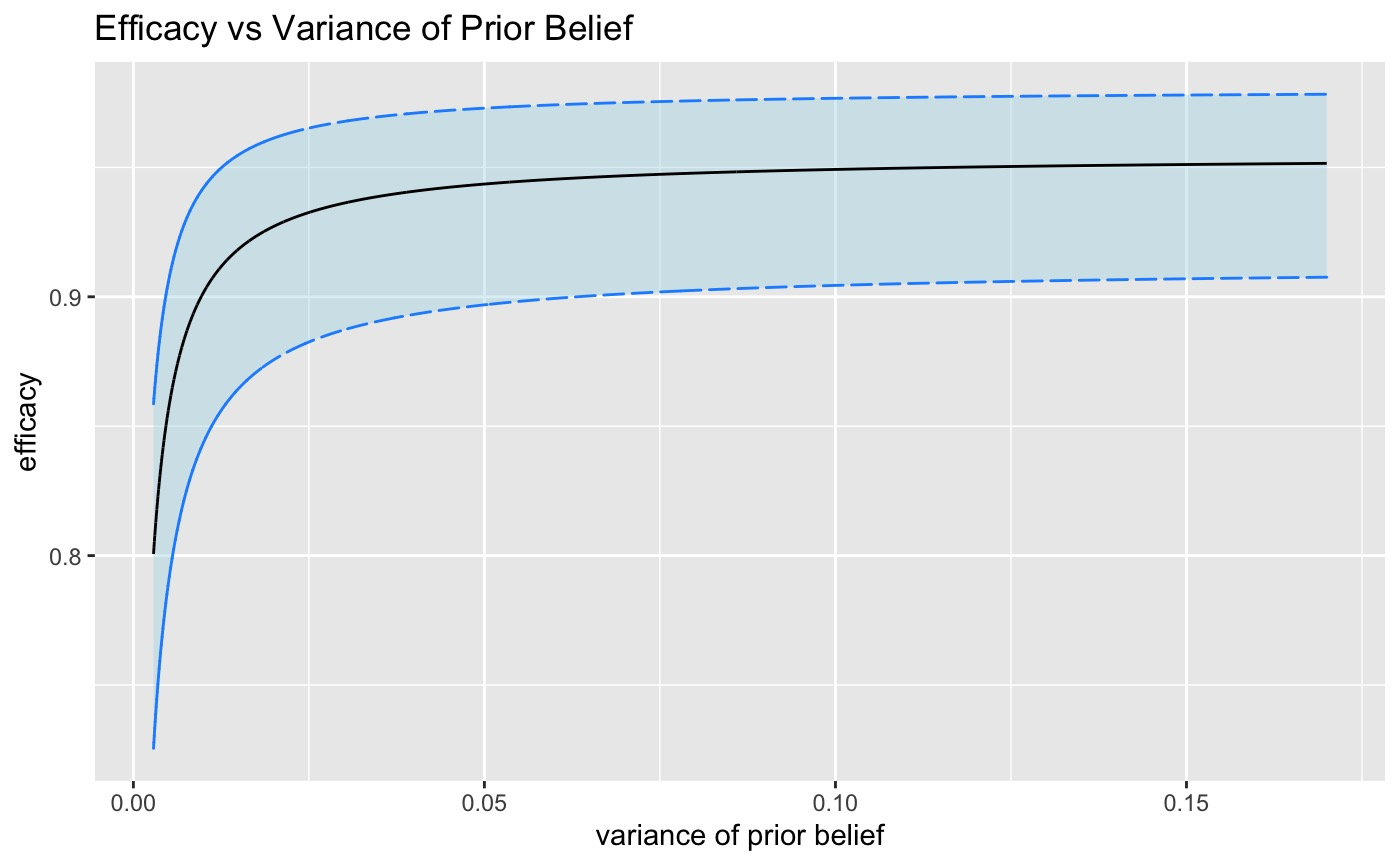
\includegraphics[width = 0.9\textwidth]{EfficacyVSVariance.jpeg}
    \caption{\footnotesize{Relationship between 95\% credible interval of vaccine efficacy and variance of the prior.}}
    \label{fig:my_label}
\end{figure}

\begin{figure}[H]
    \centering
    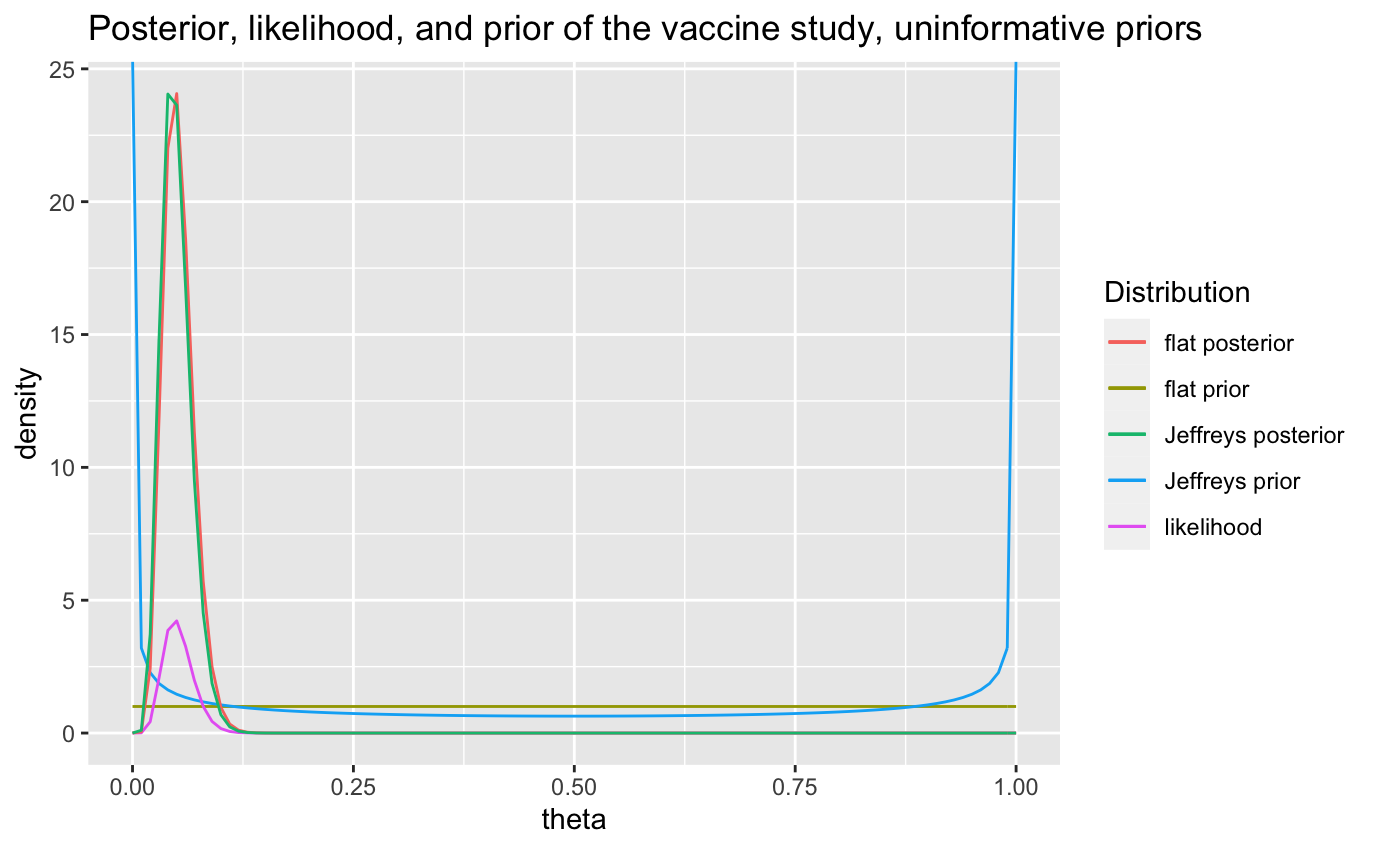
\includegraphics[width = 0.9\textwidth]{uninformative priors.png}
    \caption{\footnotesize{Posterior, likelihood, and prior of the vaccine study with uninformative priors.}}
    \label{fig: uninformative}
\end{figure}

\begin{figure}[H]
    \centering
    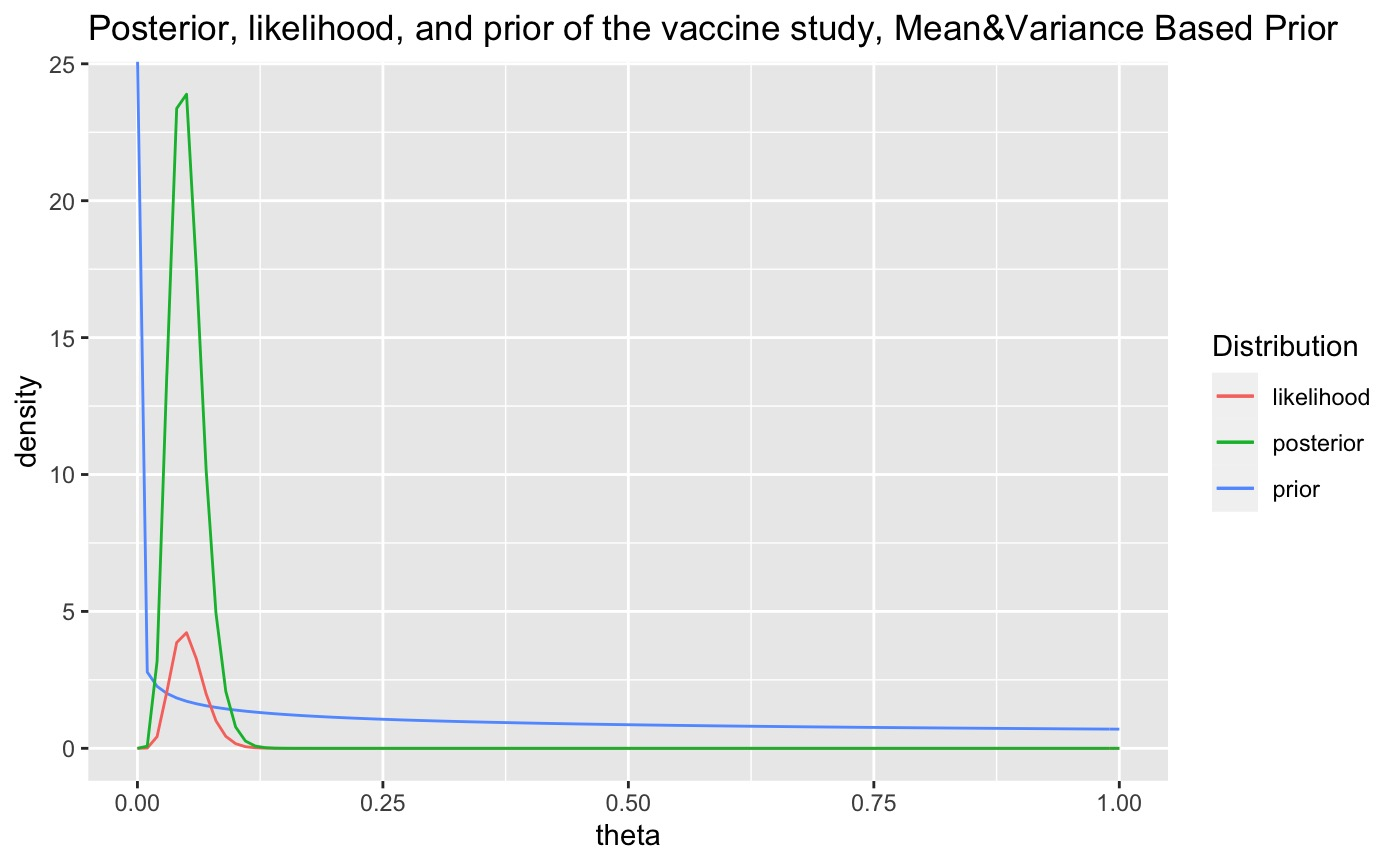
\includegraphics[width = 0.9\textwidth]{weakly informative.jpeg}
    \caption{\footnotesize{Posterior, likelihood, and prior of the vaccine study with mean \& variance based prior.}}
    \label{fig: weak}
\end{figure}

\begin{figure}[H]
    \centering
    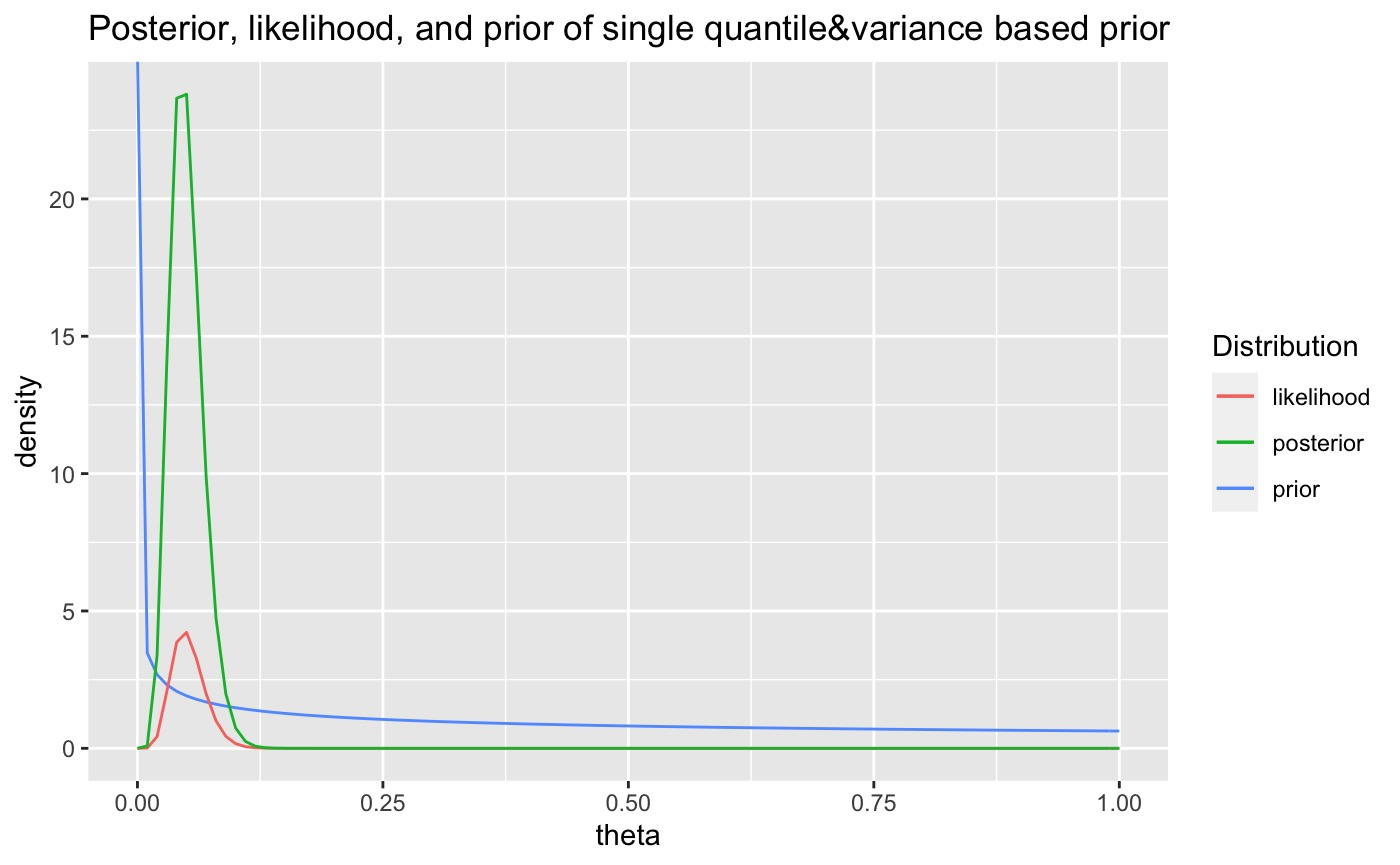
\includegraphics[width = 0.9\textwidth]{quantile approach.jpeg}
    \caption{\footnotesize{Posterior, likelihood, and prior of the vaccine study with single quantile \& variance based prior.}}
    \label{fig: quantile}
\end{figure}
\begin{figure}[H]
    \centering
    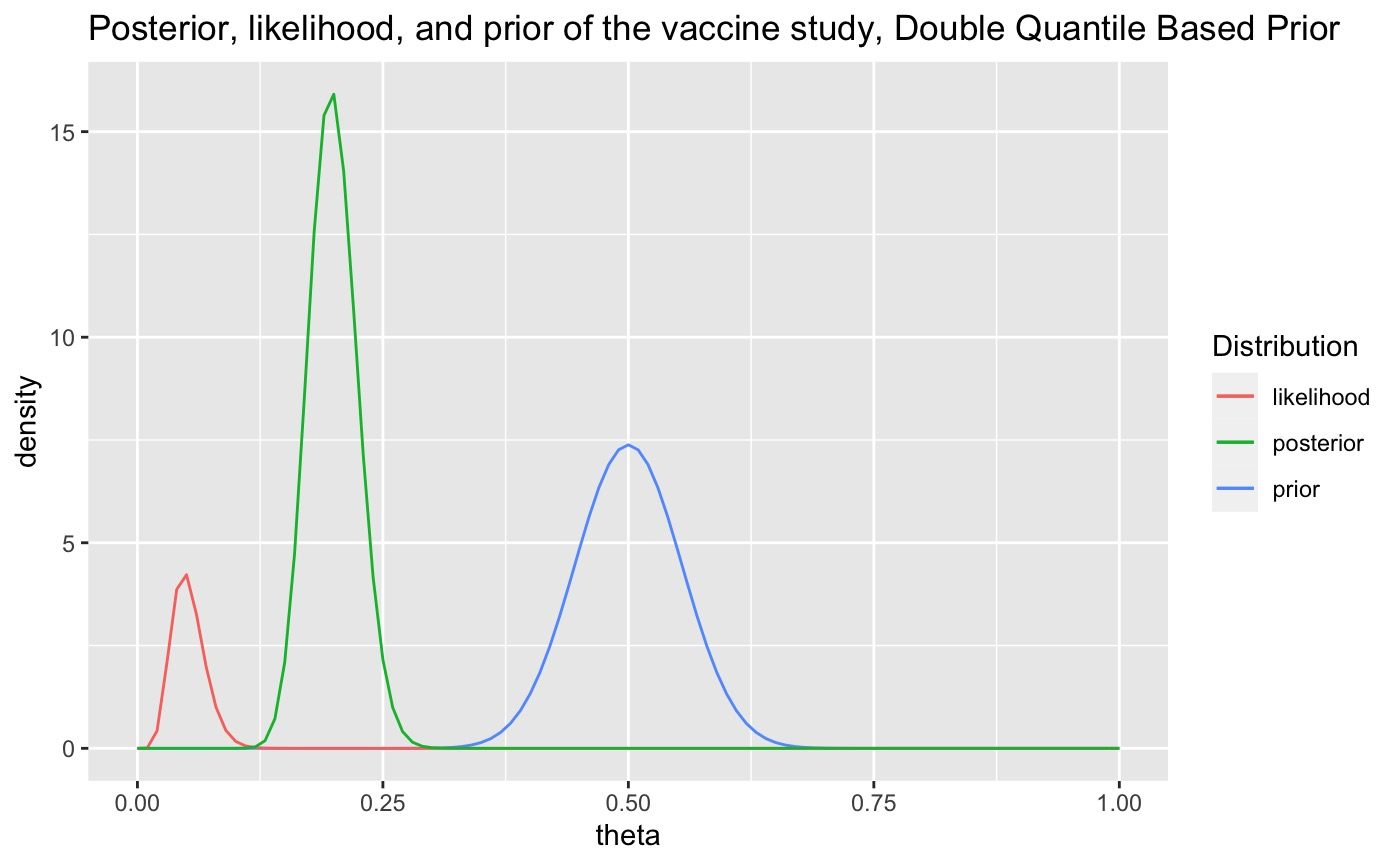
\includegraphics[width = 0.9\textwidth]{strongly informative.jpeg}
    \caption{\footnotesize{Posterior, likelihood, and prior of the vaccine study with double quantiles based prior.}}
    \label{fig: strong}
\end{figure}
\begin{figure}[H]
    \centering
    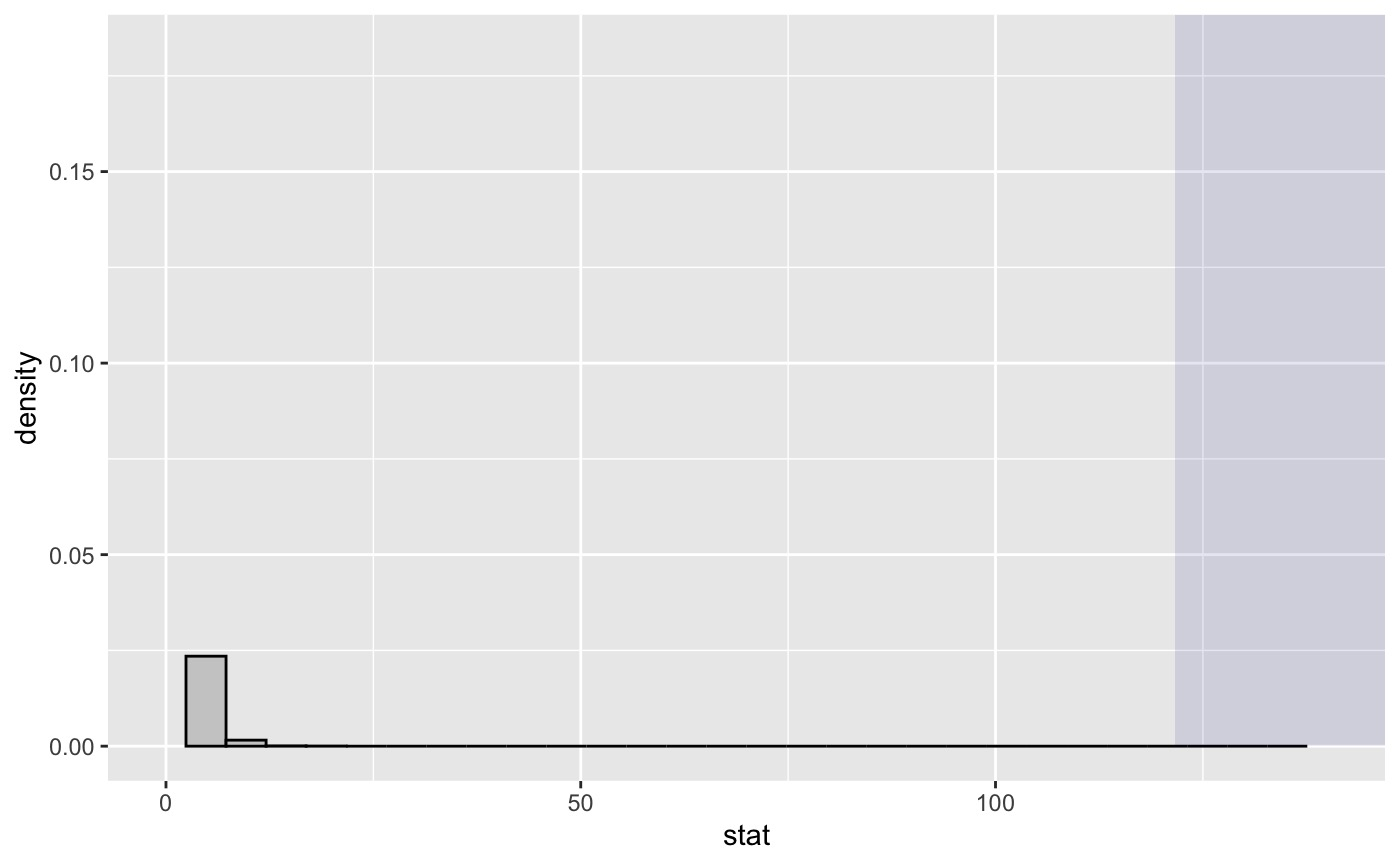
\includegraphics[width = 0.9\textwidth]{EmpiricalPVal.jpeg}
    \caption{\footnotesize{Empirical Chisq approximation.}}
    \label{fig: EmpPVal}
\end{figure}
\subsection{Codes}
\singlespacing
Transform between $\psi$ and $\theta$:
\begin{lstlisting}
    # convert from theta to psi
    topsi <- function(theta) {
      (1 - 2 * theta) / (1 - theta)
    }
    # convert from psi to theta
    totheta <- function(psi) {
      (1 - psi) / (2 - psi)
    }
\end{lstlisting}
Find $\alpha$ and $\beta$ satisfies the given quantile and variance constraint:
\label{code: grid}
\begin{lstlisting}[language=R][H]
    # grid approximation
    psi <- 0.5
    theta <- totheta(psi)
    beta_var <- function(a, b){
      a*b/((a+b)^2*(a+b+1))
    }
    
    # var = 1/8 
    var = c()
    alpha <- seq(0.384545, 0.384546, 0.000001)
    beta <- seq(0.55167, 0.5517, 0.000001)
    for(i in alpha){
      for(j in beta) {
        med = qbeta(0.5, i, j)
        var = beta_var(i, j)
        if (abs(med-theta) < 0.000001 & abs(var-1/8) < 0.000001){
          print(paste(med, var, i, j))
        }
      }
    }
\end{lstlisting}
Find credible interval for any given prior $Beta(\alpha, \beta$):
\begin{lstlisting}[language=R][H]
    a <- alpha
    b <- beta
    w <- 8
    n <- 170
    post_beta <- n - w + b
    post_alpha <- w + a
    lower <- topsi(qbeta(0.975, shape1 = post_alpha, shape2 = post_beta))
    upper <- topsi(qbeta(0.025, shape1 = post_alpha, shape2 = post_beta))
    CI <- c(lower, upper)
\end{lstlisting}
Find confidence interval for $\psi$ using multiple methods:
\begin{lstlisting}[language=R][H]
    library(mosaic)
    library(tidyverse)
    
    wald <- confint(binom.test(x = 8, n = 170, ci.method = "Wald"))
    score <- confint(binom.test(x = 8, n = 170, ci.method = "score"))
    plus4 <- confint(binom.test(x = 8, n = 170, ci.method = "Plus4"))
    cp <- confint(binom.test(x = 8, n = 170))
    
    transform.confint <- function(lower.theta, upper.theta){
          tibble(lower = (1-2*upper.theta)/(1-upper.theta), upper = (1-2*lower.theta)/(1-lower.theta))
    }
    
    wald.psi <- transform.confint(wald$lower, wald$upper)
    score.psi <- transform.confint(score$lower, score$upper)
    plus4.psi <- transform.confint(plus4$lower, plus4$upper)
    cp.psi <- transform.confint(cp$lower, cp$upper)
    psi.confint.matrix <- rbind(wald.psi, score.psi, plus4.psi, cp.psi)
    
    psi.confint.matrix$method <- c("Wald", "Wilson Score", "Plus 4", "Clopper Pearson")
    psi.confint.matrix %>% dplyr::select(method, lower, upper)
\end{lstlisting}
Code realization of Figure \ref{fig: intervals} via \texttt{ggplot2}:
\begin{lstlisting}[language=R][H]
    approaches <- c('Double Quantile', 'Polack et al. (2020)', 'Mean&Variance (var = 1/12)', 'Flat', 'Jeffreys', 'Likelihood Ratio', 'Wald', 'Clopper Pearson', 'Single Quantile&Variance')
    lowerci <- c(0.666, 0.904, 0.903, 0.901, 0.905, 0.906, 0.914, 0.900, 0.9059)
    upperci <- c(0.820, 0.976, 0.976, 0.975, 0.977, 0.978, 0.985, 0.979, 0.9775)
    median <-  c(0.752, 0.949, 0.948, 0.947, 0.950, 0.951, 0.951, 0.951, 0.9504)
    CIs <- data.frame(
      approaches <- approaches,
      lower <- lowerci,
      upper <- upperci,
      median <- median
      
     pd <- position_dodge(0.78)
    ggplot(CIs, aes(y=approaches)) +
      geom_errorbar(data=CIs, aes(xmin=lower, xmax=upper, color=approaches), width=.1, position=pd, size = 8) + 
      geom_vline(xintercept = 0.950, linetype="dashed") +
      geom_point(data=CIs, aes(x=median), position=pd) +
      xlim(0.62, 1) + 
      xlab("Efficacy") +
      ggtitle("95% Confidence/Credible Intervals for Efficacy") +
      scale_color_brewer(palette="Set3") +
      theme_bw() +
      theme(panel.border = element_blank(), panel.grid.major = element_blank(),
            panel.grid.minor = element_blank(), axis.line = element_line(colour = "black"), 
            text = element_text(size = 13), legend.position = "none") 
\end{lstlisting}

\doublespacing
\end{document}